\documentclass[main.tex,fontsize=8pt,paper=a4,paper=portrait,DIV=calc,]{scrartcl}
% Document
\usepackage[T1]{fontenc}
\usepackage[dvipsnames]{xcolor}
\usepackage[nswissgerman,english]{babel}
\renewcommand{\familydefault}{\sfdefault}

% Format
\usepackage[top=5mm,bottom=1mm,left=5mm,right=5mm]{geometry}
%\setlength{\headheight}{\baselineskip}
%\setlength{\headsep}{0mm}

%\usepackage{scrlayer-scrpage}
%\clearpairofpagestyles
%\chead{{\bfseries\TITLE, \AUTHOR, \pagename~\thepage}}

%\addtokomafont{pagehead}{\upshape}

\usepackage{multicol}
\setlength{\columnsep}{2mm}
\setlength{\columnseprule}{0.1pt}

% Math
\usepackage{amsmath}
\usepackage{amssymb}
\usepackage{amsfonts}

% Code
\usepackage{fancyvrb, etoolbox, listings, xcolor}
%\usemintedstyle{bw}

%\newminted[shell]{bash}{
%fontsize=\footnotesize,
%fontfamily=tt,
%breaklines=true,
%frame=single,
%framerule=0.1pt,
%framesep=2mm,
%tabsize=2
%}
%\newminted{css}{
%breaklines=true,
%tabsize=4,
%autogobble=true,
%escapeinside=||,
%stripall=true,
%stripnl=true,
%}

    \definecolor{lightgray}{rgb}{0.95, 0.95, 0.95}
    \definecolor{darkgray}{rgb}{0.4, 0.4, 0.4}
    \definecolor{purple}{rgb}{0.65, 0.12, 0.82}
    \definecolor{ocherCode}{rgb}{1, 0.5, 0} % #FF7F00 -> rgb(239, 169, 0)
    \definecolor{blueCode}{rgb}{0, 0, 0.93} % #0000EE -> rgb(0, 0, 238)
    \definecolor{greenCode}{rgb}{0, 0.6, 0} % #009900 -> rgb(0, 153, 0)
    \definecolor{teal}{rgb}{0.0, 0.5, 0.5}

\lstdefinestyle{code}{
    identifierstyle=\color{black},
    keywordstyle=\color{blue}\bfseries\small,
    ndkeywordstyle=\color{greenCode}\bfseries\small,
    stringstyle=\color{ocherCode}\ttfamily\small,
    commentstyle=\color{teal}\ttfamily\textit\small,
    basicstyle=\ttfamily\small,
    breakatwhitespace=false,         
    breaklines=true,                 
    captionpos=b,                    
    keepspaces=true,                 
    showspaces=false,                
    showstringspaces=false,
    showtabs=false,                  
    tabsize=2,
    belowskip=-5pt
}



% Images
\usepackage{graphicx}
\newcommand{\pic}{\includegraphics[scale=0.3]}
\graphicspath{{Screenshots/}{../Screenshots}}
\makeatletter
\def\pictext#1#2{%
    \@ifnextchar[{%
    \pictext@iiiii{#1}{#2}%
    }{%
      \pictext@iiiii{#1}{#2}[0.5,0.4,0.3]% Default is 5
    }%
}
\def\pictext@iiiii#1#2[#3,#4,#5]{\begin{minipage}{#3\textwidth}\includegraphics[scale=#4]{#1}\end{minipage}\begin{minipage}{#5\textwidth}#2\end{minipage}}
\def\minipg#1#2{%
    \@ifnextchar[{%
    \minipg@iiii{#1}{#2}%
    }{%
      \minipg@iiii{#1}{#2}[0.3,0.6]% Default is 5
    }%
}
\def\minipg@iiii#1#2[#3,#4]{\vspace{0.8mm}\begin{minipage}{#3\textwidth}#1\end{minipage}\begin{minipage}{#4\textwidth}#2\end{minipage}{\vspace{0.8mm}}}
\makeatother

%\newenvironment{minty}[2]% environment name
%{% begin code
%  \begin{minipage}{#1}
%  \begin{minted}{#2}
%}%
%{% end code
%  \end{minted}
%  \end{minipage}
%  \end{minty}\ignorespacesafterend
%} 

% Smaller Lists
\usepackage{enumitem}
\setlist[itemize,enumerate]{leftmargin=3mm, labelindent=0mm, labelwidth=1mm, labelsep=1mm, nosep}
\setlist[description]{leftmargin=0mm, nosep}
\setlength{\parindent}{0cm}

% Smaller Titles
\usepackage[explicit]{titlesec}

%% Color Boxes
\newcommand{\sectioncolor}[1]{\colorbox{black!60}{\parbox{0.989\linewidth}{\color{white}#1}}}
\newcommand{\subsectioncolor}[1]{\colorbox{black!50}{\parbox{0.989\linewidth}{\color{white}#1}}}
\newcommand{\subsubsectioncolor}[1]{\colorbox{black!40}{\parbox{0.989\linewidth}{\color{white}#1}}}
\newcommand{\paragraphcolor}[1]{\colorbox{black!30}{\parbox{0.989\linewidth}{\color{white}#1}}}
\newcommand{\subparagraphcolor}[1]{\colorbox{black!20}{\parbox{0.989\linewidth}{\color{white}#1}}}

%% Title Format
\titleformat{\section}{\vspace{0.5mm}\bfseries}{}{0mm}{\sectioncolor{\thesection~#1}}[{\vspace{0.5mm}}]
\titleformat{\subsection}{\vspace{0.5mm}\bfseries}{}{0mm}{\subsectioncolor{\thesubsection~#1}}[{\vspace{0.5mm}}]
\titleformat{\subsubsection}{\vspace{0.5mm}\bfseries}{}{0mm}{\subsubsectioncolor{\thesubsubsection~#1}}[{\vspace{0.5mm}}]
\titleformat{\paragraph}{\vspace{0.5mm}\bfseries}{}{0mm}{\paragraphcolor{\theparagraph~#1}}[{\vspace{0.5mm}}]
\titleformat{\subparagraph}{\vspace{0.5mm}\bfseries}{}{0mm}{\subparagraphcolor{\thesubparagraph~#1}}[{\vspace{0.5mm}}]

%% Title Spacing
\titlespacing{\section}{0mm}{0mm}{0mm}
\titlespacing{\subsection}{0mm}{0mm}{0mm}
\titlespacing{\subsubsection}{0mm}{0mm}{0mm}
\titlespacing{\paragraph}{0mm}{0mm}{0mm}
\titlespacing{\subparagraph}{0mm}{0mm}{0mm}

%% format cells
\usepackage[document]{ragged2e}
\usepackage{array, makecell}
\renewcommand{\arraystretch}{2}
\newcommand{\mc}{\makecell[{{m{1\linewidth}}}]}



\lstset{
    language=c++,
    style=code,
}
%%%%%

\begin{document}
\begin{table}[h!]
\section{Basic Terms and Information}
\begin{tabular}{|m{0.2\linewidth}|m{0.755\linewidth}|}
\hline
Preprocessor & Handles the \#include or \#def commands. Essentially loads these includes and places them where needed. Files after this stage have the .i notation -> main.i \\
\hline
Compiler & Turns the Code into an executable. Note that libraries are not automatically included here. Files after this stage have the .o notation -> main.o \\
\hline
Linker & Indluces the libraries at the end and puts them into the executable. This is used to run this binary on a pc without these libraries installed. Files after this stage no longer have a special notation. \\
\hline
\textbf{\emph{Declaration}}
&
This only declares the variable, it does not have a predefined value -> undefined behavior!\newline
\begin{lstlisting}
int i;
char c;
\end{lstlisting}
\\
\hline

\textbf{\emph{Definition}}
&
This defines a variable with a set value.\newline
\begin{lstlisting}
int i = 5;
int a{5};
\end{lstlisting} 
\, \newline
\textcolor{red}{\textbf{PLEASE, note the \emph{extern} keyword}}\newline
\textcolor{orange}{This means that only a tag is declared, there is no memory allocation yet.\newline
Without extern the memory is allocated, this is as the extern expects the variable to be declared/defined somewhere else}\\
\hline

\textbf{\emph{Variables close to usage}}
&
\pic{2022-09-27-08:41:06.png}\\
\hline
\end{tabular}
\subsection{Preprocessor Commands:}
\begin{tabular}{|m{0.2\linewidth}|m{0.755\linewidth}|}
\hline
\#ifdef / \#ifndef \newline \#define \newline \#endif & These are used to check if things are already defined, or to define them. Either for checks to avoid double definition, or to check if debug is used -> ifdef DEBUG\\
\hline
Include differences & \#include <library> \textcolor{teal}{search in the system include directories!}\newline
\#include "library" \textcolor{teal}{search in the current working directory, \textbf{AND after that in the system includes}}\\
\hline
\#pragma once & This is used to automatically avoid double include statements. Aka if it is included already simply ignore any double includes. \\
\hline
\textbf{Macros simple object version} & 
\#define XYZ 123 \newline
int x = XYZ compiles to int x = 123\\
\hline
\textbf{Cmake} & cmake -B build | this will define the directory to build in \newline cmake --build directory | this will build the system into this directory \newline cmake . | creates the CMakeFile and other files inside the specified director
\\
\hline
\textbf{General Rule} & \emph{Only include what's necessary, don't just generalize includes to include everything!}\\
\hline
\end{tabular}
\section{Value Interpretation}
\begin{tabular}{|m{0.975\linewidth}|}
\hline
\pic{2022-09-27-08:47:15.png}
\\
\hline
\end{tabular}
\end{table}
\pagebreak
\begin{table}[h!]
\section{Basic Syntax and Keywords}
\begin{tabular}{|m{0.4\linewidth}|m{0.555\linewidth}|}
\hline
\begin{lstlisting}
const int i = 5;
\end{lstlisting}
&
Const simply defines a variable that is immutable.
\\

\hline
\begin{lstlisting}
void toUpper(std::string & value) {
    for (char & c : value) {
        c = toupper(c);
    }
}
\end{lstlisting}
&
This is cool as it actually changes the stuff inside a for-loop with ranges.\newline
RIGHT JAVA?
\\

\hline
\begin{lstlisting}
std::array<int, 5> arr{1,2,3,4,5};
int arr[]{1,2,3,4,5};
//both work
\end{lstlisting}
& \minipg{Fixed size arrays.\newline Faster than vector but not dynamic.}
{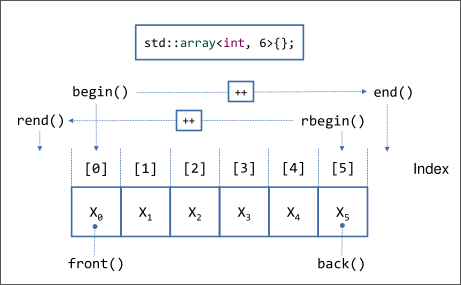
\includegraphics[scale=0.4]{2022-10-04-08:41:42.png}}[0.2,0.5]\\

\hline
\begin{lstlisting}
std::vector<int> arr{1,2,3,4,5};
std::vector arr{1,2,3,4,5}; 
//if elements are provided, then type can be omitted.
std::vector<int>(6); 
//int vector with size 6, with all elements being 0 -> default.
vector.push_back(element); //insert at end
vector.insert(pos,element); //insert at iterator
vector.erase(iterator); 
//vector.begin() vector.end()
vector.front();
vector.back();
vector.find(element);
\end{lstlisting}
& \minipg{Vector are simply the dynamic default datastructure in c++.\newline
\textbf{\textcolor{red}{Index variable type is unsigned int >> size\_t or std::vector<T>::size\_type}}\newline
\textbf{Iterating through a vector without at() is unsafe, \newline it will cause undefined behavior if out of bounds.\newline
With at() it will cause an exception instead.}}
{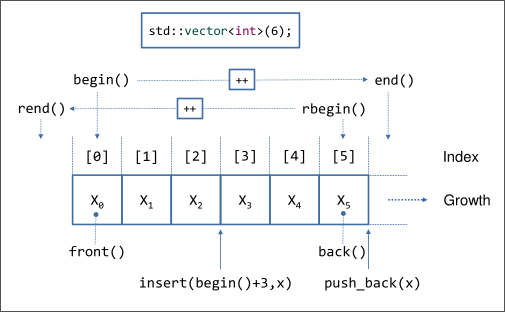
\includegraphics[scale=0.4]{2022-10-04-08:48:54.png}}[0.2,0.5]
\\

\hline
\begin{lstlisting}
[<capture>](<parameters>) -> <return-type> {
<statements>
}
\end{lstlisting}
& Basic Lambda syntax\newline
If you capture a value by value then it is by default const.\newline
 References, aka referenced pointer is handled with the \& symbol.
\\
\hline
\begin{lstlisting}
auto zero_it = std::find(std::begin(v), std::end(v), 0);
if (zero_it == std::end(v)){
std::cout << "no zero found \n";
}
\end{lstlisting}
&

\\

\hline
\begin{lstlisting}
std::vector<int> v{5, 4, 3, 2, 1};
std::cout << std::accumulate(std::begin(v), std::end(v), 0)<< " = sum\n";

void printDistanceAndLength(std::string s) {
std::cout << "distance: "<< std::distance(s.begin(), s.end()) <<'\n';
std::cout << "in a string of length: "<< s.size()<<'\n';
}
\end{lstlisting}
& diverse standard library iteration and loops.
\\

\hline
\begin{lstlisting}
void print(int x) {
std::cout << "print: "<< x << '\n';
}
void printAll(std::vector<int> v) {
std::for_each(std::crbegin(v), std::crend(v), print);
}
\end{lstlisting}
& For each loop\\
\hline
\textbf{Function Overloading}\newline
\begin{lstlisting}
void incr(int & var);
void incr(int & var, unsigned delta);
\end{lstlisting}
& Will always use the more specific function.\newline
\textcolor{red}{Be aware that you should always make sure you enter the type that you want!\newline
Don't do automatic casting for overloaded functions!}\\
\hline
\textbf{Default Values}\newline
\begin{lstlisting}
void incr(int & var, unsigned delta = 1);
void incr(int & var, unsigned delta) {
var += delta;
}
\end{lstlisting}
& \textcolor{teal}{Amazing functionality! This means that you can create \textbf{optional parameters!}}\\
\hline
\textbf{Alias}\newline
\begin{lstlisting}
using <alias> = <type>;
\end{lstlisting}
& Just don't do using namespace std;\\
\hline
\end{tabular}
\end{table}
\pagebreak
\begin{table}[ht!]
\begin{tabular}{|m{0.2\linewidth}|m{0.755\linewidth}|}
\hline
\textbf{Lambda and std::function}\newline
\begin{lstlisting}
// std::function
std::function<double(double)>

// lambda 
auto some_func = [dependency](paremeter) {};
\end{lstlisting}
& Example for lambda:\newline
\begin{lstlisting}
int main() {
  double factor{3.0};
  auto const multiply = [factor](double value) {
    return factor * value;
  };
  applyAndPrint(1.5, multiply);
}

// create a new variable instead of capturing it
// can only be modified with mutable
// variable has type auto
auto squares = [x=1]() mutable {
std::cout << x *= 2;
};

// this pointer in lambda
struct S {
void foo() {
auto square = [this] {
member *= 2;
};
}
private:
int member{};
};
\end{lstlisting}
\, \newline
\textcolor{teal}{\char`\[  \char`\] These capture a variable from scope.}\newline
\textcolor{teal}{With brackets a variable can also be captured by reference -> \char`[ \&x\char`]}\newline
\textcolor{teal}{The \textcolor{red}{this} keyword can also be captured}\newline
\textcolor{teal}{\char`\( \char`\) These are for parameters just like a normal function}\\
\hline
\textbf{auto function return}\newline
\begin{lstlisting}
auto middle(std::vector<int> const & c) {
//check not empty
return c[c.size() / 2];
}
\end{lstlisting}
& This can automatically deduce the type, problem is,\newline
it might not show the type for every IDE.\newline
\textcolor{red}{The function body must be present for this!}\\
\hline
\textbf{static} &
\textcolor{orange}{static inside a function}\newline
\begin{lstlisting}
void spass() {
  static int x = 5;
  x++;
  std::cout << x << "\n";
}
\end{lstlisting}
\, \newline
\textcolor{orange}{This would increment x everytime you call this function with only defining it once!\newline
This even applies when you call this function from multiple sources}\\
\hline
\textbf{Inline} & 
\textcolor{orange}{Inline is used to define a function inside a header file, \newline
this is usually only done with operator overloading in header files}\newline
\begin{lstlisting}
class Date {
int year, month, day;
public:
auto operator<(Date const& right) const -> bool;
};

inline auto operator>(Date const& left, Date const& right) -> bool {
return right < left;
}
\end{lstlisting}\\
\hline
\end{tabular}
\end{table}
\pagebreak
\begin{table}[ht!]
\section{Best practices}
\begin{tabular}{|m{0.2\linewidth}|m{0.755\linewidth}|}
\hline
\textbf{Const by default} & 
\textcolor{red}{It is general best practice to always use const unless mutability is necessary!}\newline
\pic{2022-10-11-08:36:02.png}\\
\hline
\end{tabular}
\end{table}
\pagebreak
\begin{table}[h!]
\section{Default Operators}
\begin{tabular}{|m{0.2\linewidth}|m{0.755\linewidth}|}
\hline
\begin{lstlisting}
|| && == <= >= != > <
\end{lstlisting}
&
OR, AND, equals, smaller than or equals, greater than or equals, not equals, greater than, smaller than\\
\hline

\begin{lstlisting}
& | ^ >> <<
\end{lstlisting}
&
Bit operators.\\
\hline

\begin{lstlisting}
(5 > 4) ? true : false
\end{lstlisting}
&
Ternary Operator, or otherwise called inline if.\\
\hline
\end{tabular}
\section{Quirks}
\begin{tabular}{|m{0.25\linewidth}|m{0.705\linewidth}|}
\hline
\begin{lstlisting}
double f = 45 / 8;
\end{lstlisting}
&
In math operations the actual number takes precedence, here the numbers are int, therefore the value will be truncated to 5. If you want double or float division use 45.0 / 8.0 or 45.f / 8.f. \\
\hline
\textbf{\emph{Accessing Containers}} & 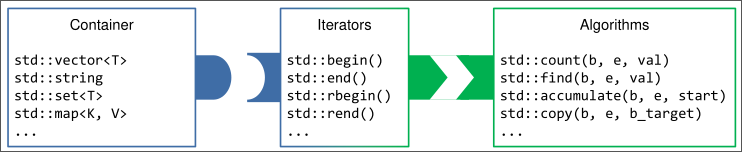
\includegraphics[scale=0.4]{2022-10-04-09:40:48.png}\\
\hline
\end{tabular}
\section{IO-Streams}
\begin{tabular}{|m{0.25\linewidth}|m{0.705\linewidth}|}
\hline
\begin{lstlisting}
std::ostream / std::istream
\end{lstlisting}
&
These represent the system IO, and they do therefore not have a value.\newline
This means you can't copy these, you can only pass references/pointers.
\\
\hline

\begin{lstlisting}
.clear() and .good()
\end{lstlisting}
&
If you use the streams yourself, aka not std::cout or std::cin, then you have to deal with the problems that can occur with it.\newline
This means that you have to check whether or not the stream is valid with .good() and clear it with .clear() should an error occur. \newline
Otherwise the stream will not be cleared for the next usage.
\\
\hline

\begin{lstlisting}
int inputAge(std::istream& in) {
    int age{-1};
    if (in >> age) {
        return age;
    }
    return -1;
}
\end{lstlisting}
&
Here the in >> age will return true if the input was successfully transferred into the stream.
\\
\hline
\textbf{\emph{\textcolor{red}{Terminating Inputstreams}}}
&
Terminating inputstreams can be done with \textbf{\emph{\textcolor{red}{CTRL+D}}}\\
\hline
Stream states & \vspace{2mm}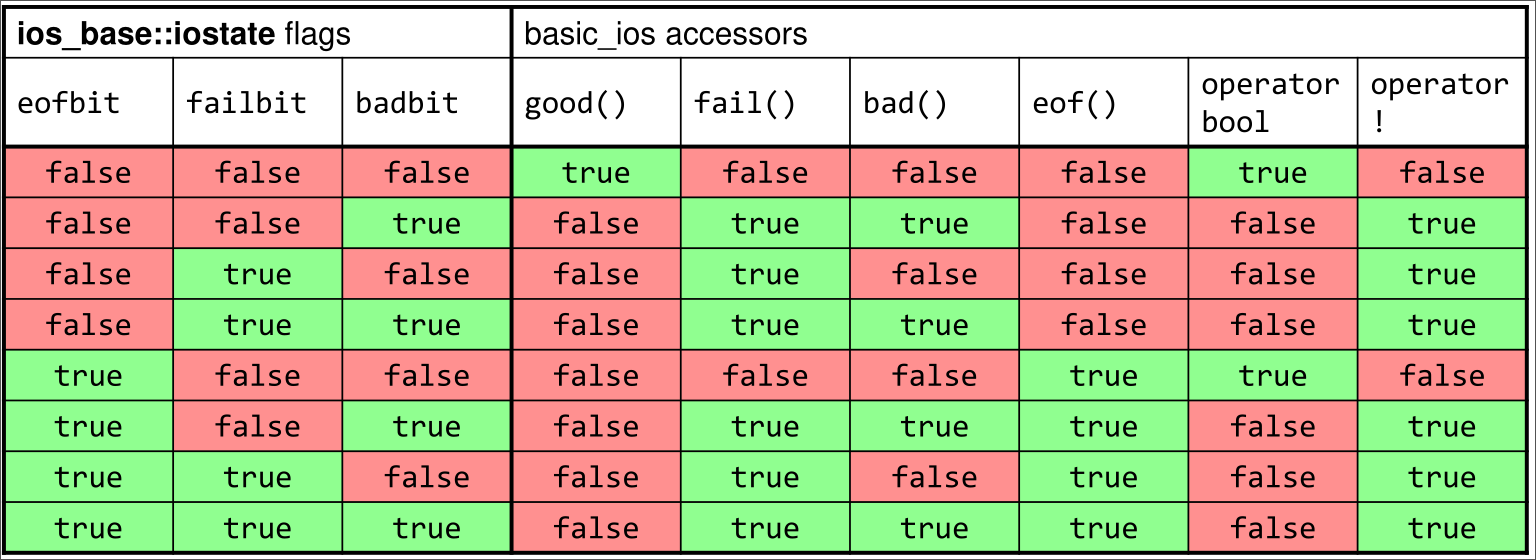
\includegraphics[scale=0.25]{2022-10-04-08:13:36.png} \\
\hline
\emph{Formatting} &
\vspace{2mm}
\begin{itemize}
  \item std::cout << std::oct << number;
  \item std::cout << std::hex << number;
  \item std::cout << std::dec << number;\newline
    \textcolor{red}{These are sticky, meaning this formatting will stick from that line on.}\newline
  \item std::setprecision 
  \item std::fixed 
  \item std::scientific
  \item std::left
  \item std::setw(10) //output at least 10 digits long
\vspace{-3mm}
\end{itemize}
\\
\hline
\end{tabular}
\section{Loops}
\begin{tabular}{|m{0.25\linewidth}|m{0.705\linewidth}|}
\hline
\textbf{\emph{Range based for-loop}}
& 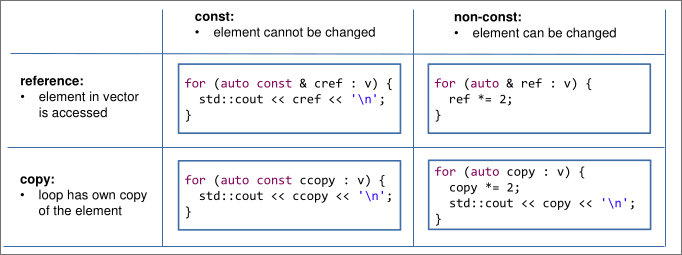
\includegraphics[scale=0.4]{2022-10-04-09:19:47.png}\\
\hline
\textbf{\emph{Iterator based for-loop}}
& \minipg{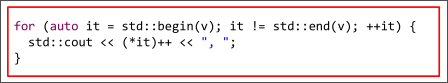
\includegraphics[scale=0.4]{2022-10-04-09:24:39.png}\newline non constant}
{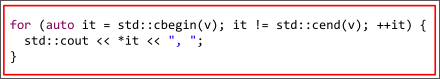
\includegraphics[scale=0.4]{2022-10-04-09:24:44.png}\newline constant}[0.4,0.5]\\
\hline
\end{tabular}
\end{table}
\pagebreak
\begin{table}[ht!]
\section{Pointer and References}
\begin{tabular}{|m{0.2\linewidth}|m{0.755\linewidth}|}
\hline
\textbf{Returning References}\newline
\begin{lstlisting}
// ok
std::ostream & sayHello(std::ostream & out) {
return out << "Hello";
}

// No 
std::string & create() {
std::string name{"John"};
return name;
}
\end{lstlisting}
& 
You can return references, but keep in mind that this basically means returning a pointer.\newline
If you create a variable and return a reference to it, then that pointer is now invalid!\newline
\textcolor{red}{Accessing an invalid pointer will cause a segmentation fault!}\\
\hline
\end{tabular}
\begin{tabular}{|m{0.2\linewidth}|m{0.755\linewidth}|}
\hline

\hline
\end{tabular}
\section{Cmake}
\begin{tabular}{|m{0.2\linewidth}|m{0.755\linewidth}|}
\hline
\textbf{ClangD LSP include} & 
In order to include your projects in the clanD server, you need to compile a json file with cmake.\newline
\large\textbf{\textcolor{teal}{cmake -DCMAKE\_EXPORT\_COMPILE\_COMMANDS=1}}\newline
\normalsize After this command everything will be setup for your to start programming with all the whistles that you need.\\
\hline
\end{tabular}
\section{Error Handling}
\begin{tabular}{|m{0.2\linewidth}|m{0.755\linewidth}|}
\hline
\textbf{Ways to handle Errors} &
\begin{enumerate}
  \item Ignore the error and provide a potentially \textcolor{red}{undefined behavior}
  \item Return a \textcolor{red}{standard result} to cover the error
  \item Return an \textcolor{red}{error code} or error value
  \item Provide an \textcolor{red}{error status} as a side-effect
  \item Throw an \textcolor{red}{exception} -> perfomance heavy
\end{enumerate}\\
\hline
Ignoring an error & 
Example\newline
\begin{lstlisting}
std::vector v{1, 2, 3, 4, 5};
v[5] = 7;
\end{lstlisting}
\, \newline
\begin{itemize}
  \item Relies on the caller to satisfy all preconditions
  \item Viable only if not dependent on other resources
  \item Most efficient implementation\newline
   No unnecessary checks
  \item Simple for the implementer but harder for the caller
  \item Should be done consciously and consistently!
\end{itemize}
\\
\hline
Cover an Error & 
\begin{lstlisting}
int div(int number, int number2) {
  if(number2 == 0) {
    return 0;
  }
  return number / number2;
}
\end{lstlisting}
\, \newline
This is bad as it can lead to strange behavior in debugging, but is performant!\\
\hline
Error Value with std::optional & 
\begin{lstlisting}
std::optional<std::string> inputName(std::istream & in) {
  std::string name{};
  if (in >> name) return name;
  return {};
}
\end{lstlisting}
\, \newline
\textcolor{teal}{This simply returns the type string if name was able to be parsed, or no type, aka void if it could not be parsed.}\\
\hline
Error Status Side Effect &

\\
\hline
Exceptions & 
\begin{lstlisting}
throw std::some_exception{"error text"};
throw ExceptionName;
throw ENUM;

// don't
throw 2;
throw "sowwy ewwow";
\end{lstlisting}
\, \newline
With C++ you can throw all kinds of crap, but please, throw exceptions or enums.\\
\hline
\end{tabular}
\end{table}
\pagebreak
\begin{table}[ht!]
\section{Classes and Structs}
\begin{tabular}{|m{0.2\linewidth}|m{0.755\linewidth}|}
\hline
Classes &
\textcolor{orange}{Classes and Structs are defined like this:}\newline
\begin{lstlisting}
class Something { 
public:
// default for struct
// visible for everyone
static int returnValue();
// static simply means that you can use this function without an instance!
protected:
// visible only to class and subclasses
private:
// default for classes
// visible only for class
};
\end{lstlisting}
\, \newline
\textcolor{teal}{Other than the private and public denotations, structs are defined the same way, and also operate the same way!}\\
\hline
\textbf{Initializer List\newline and Constructor} & 
\begin{lstlisting}
class Something {
private:
  int a,b;
public:
  Something(int a, int b);
}

Something(int a, int b) : 
a{a}, b{b} {
// regular constructor
// !! a constructor doesn't return a value !!
}
\end{lstlisting}
\, \newline
\textcolor{teal}{C++ has a default constructor -> Something()}\newline
\textcolor{orange}{\textbf{A constructor does not return a value!}}\\
\hline
\textbf{Copy and Move Constructor} & 
\begin{lstlisting}
Date d{};
Date d2{d};
// copies d into d2
// 2 instances now!
Date d3{std::move(d)};
// move constructor!
// this moves the values of d into d3, 1 instance only!
\end{lstlisting}
\, \newline
\begin{lstlisting}
Date() = default; // default constructor, if you write this, write default to avoid overwriting it!
Date(Date const &); // copy constructor
Date(Date &&); // move constructor
\end{lstlisting}
\\
\hline
\textbf{default values in Constructors} & 
\begin{lstlisting}
explicit Date(int year, int month = 1, int day = 1);
// explicit means that we do not want implicit conversion -> double to int
// We can now call this constructor with either 1, 2 or 3 parameters, as 2 of them have a default value!
\end{lstlisting}
\\
\hline
List Constructor with Containers & 
\begin{lstlisting}
std::vector(5,10);
// creates a vector with 5 elements of value 10!
// same as -> std::vector(std::initializer_list<5> 10);

std::vector{5,10};
// creates a vector with element 5 and 10!
\end{lstlisting}\\
\hline
\textbf{Destructor} & 
\begin{lstlisting}
~Date();
// do something before we delete this instance
\end{lstlisting}
\, \newline
\textcolor{orange}{\textbf{This may never throw an exception!}}\\
\hline
\textbf{Inheritance} & 
\begin{lstlisting}
class SubDate : public Date { 
// public -> keep as is
// protected -> change all public to protected -> not directly accessible
// private -> change all inherited to private -> not directly accessible
// default inheritance is based on class or strcut -> private and public
};

class SubDate2 : public SubDate, public Date {
// ...
};
\end{lstlisting}
\, \newline
\textcolor{teal}{A class can inherit from 1 \textbf{OR MORE} classes!}\\
\hline
\textbf{Scope} & 
\textcolor{orange}{Scope is denoted with the :: operators -> Calculator::negate(); \newline call the static function negate form Calculator}\\
\hline
Calling SuperClass Constructors & 
\begin{lstlisting}
Something() : ParentOfSomething() {
/ ...
}
// or you can call another constructor of the same element!
Something() : Something() {
/ ...
}
\end{lstlisting}
\, \newline
\textcolor{orange}{Unlike java, here we can just call constructors of multiple parent classes!}\\
\hline
const this & 
\textcolor{orange}{\textbf{The this keyword can be const, it may then not change the values of membervariables!}}\\
\hline 
\textbf{static variables} &
\begin{lstlisting}
static const Date myDate;
// this is an immutable global variable that can be accessed (read-only) with SomeThing::myDate;
static Date myOtherDate;
// this can be accessed and also changed, it is a mutable global variable!!
\end{lstlisting}
\, \newline
\textcolor{orange}{Avoid using static to create global variables if you can, this would most likely end badly.}\\
\hline
\end{tabular}
\end{table}
\pagebreak
\begin{table}[ht!]
\section{Operator Overloading}
\begin{tabular}{|m{0.2\linewidth}|m{0.755\linewidth}|}
\hline
All overloadable Operators &
\vspace{2mm}
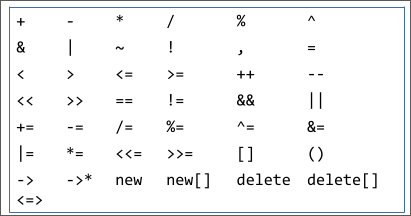
\includegraphics[scale=0.35]{2022-10-18-09:26:28.png}\\
\hline
\textbf{NON-Overloadable} Operators & 
\vspace{2mm}
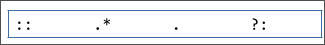
\includegraphics[scale=0.4]{2022-10-18-09:26:34.png}\\
\hline
Spaceship Operator &
\textcolor{orange}{The spaceship operator implements the usual comparison operators for you class\newline
This means <, >, <=, >=,== ,!=}\newline
\begin{lstlisting}
class Date {
int year, month, day;
public:
auto operator<=>(Date const& right) const -> std::strong_ordering {
if (year != right.year) {
return year <=> right.year;
}
if (month != right.month) {
return month <=> right.month;
}
return day <=> right.day;
}
auto operator==(Date const& right) const -> bool {
return (*this <=> right) == std::strong_ordering::equal;
} //Also allows != comparison
};
\end{lstlisting}
\, \newline
\textcolor{red}{Since C++ 20 you can also use the following to default the <=> operator}\newline
\begin{lstlisting}
class Date {
int year, month, day;
public:
auto operator<=>(Date const& right) const = default;
};
\end{lstlisting}
\\
\hline
Defaulting Operator & 
Just like with the <=> Operator you can default other operators: \newline
\begin{lstlisting}
class Point {
int x, y;
public:
auto operator==(Date const& right) const = default;
};
\end{lstlisting}\\
\hline
\textbf{Strong Ordering with <=>} &
\textcolor{teal}{Usually used with ints or Dates}\newline
\textcolor{red}{\textbf{All values are indistinguishable}}\newline
\textcolor{orange}{\textbf{one of: a > b, a == b, a < b must be true}}\newline
\begin{lstlisting}
auto operator<=>(Date const& right) const -> std::strong_ordering;
\end{lstlisting}
\, \newline
A list of possibilities:\newline
\begin{itemize}
  \item \textcolor{teal}{std::strong\_ordering::less} \,\,-> a < b 
  \item \textcolor{teal}{std::strong\_ordering::equal}\,\,-> a == b 
  \item \textcolor{teal}{std::strong\_ordering::greater}\,-> a > b 
  \vspace{-3mm}
\end{itemize}\\
\hline
\textbf{Weak Ordering with <=>} &
\textcolor{teal}{Usually used with words, -> case insenstivive -> hello == Hello}\newline
\textcolor{red}{\textbf{All values may be distinguishable}}\newline
\textcolor{orange}{\textbf{one of: a > b, a == b, a < b must be true}}\newline
\begin{lstlisting}
auto operator<=>(Date const& right) const -> std::weak_ordering;
\end{lstlisting}
\, \newline
A list of possibilities:\newline
\begin{itemize}
  \item \textcolor{teal}{std::weak\_ordering::less} \,\,-> a < b 
  \item \textcolor{teal}{std::weak\_ordering::equivalent}\,\,-> a == b 
  \item \textcolor{teal}{std::weak\_ordering::greater}\,-> a > b 
  \vspace{-3mm}
\end{itemize}\\
\hline
\textbf{Partial Ordering with <=>} &
\textcolor{teal}{Usually used with values that can be something like NaN!}\newline
\textcolor{red}{\textbf{All values may be distinguishable}}\newline
\textcolor{orange}{\textbf{a > b, a == b , a < b can all be false}}\newline
\begin{lstlisting}
auto operator<=>(Date const& right) const -> std::partial_ordering;
\end{lstlisting}
\, \newline
A list of possibilities:\newline
\begin{itemize}
  \item \textcolor{teal}{std::partial\_ordering::less} \,\,-> a < b 
  \item \textcolor{teal}{std::partial\_ordering::equivalent}\,\,-> a == b 
  \item \textcolor{teal}{std::partial\_ordering::greater}\,-> a > b
  \item \textcolor{teal}{std::partial\_ordering::unordered}\,-> non of the above
  \vspace{-3mm}
\end{itemize}\\
\hline
\end{tabular}
\end{table}
\pagebreak
\begin{table}[ht!]
\begin{tabular}{|m{0.2\linewidth}|m{0.755\linewidth}|}
\hline
Inline Operator &
\textcolor{orange}{The best way to define an operator is with the inline version:}\newline
\begin{lstlisting}
class Date {
    int year, month, day;
  public:
    auto print(std::ostream & os) const -> std::ostream& {
    //print logic
    }
};
Inline auto operator<<(std::ostream & os, Date const& date) -> std::ostream& {
  return date.print(os);
}
\end{lstlisting}
\, \newline
\textcolor{teal}{This makes sure that the operator function that is outside of your class can have any order of variables -> inside the class it would always be the "this" keyword first.\newline
However it also makes sure that the operator function respects the private variables -> no access since outside of class}\\
\hline
+= and + &
\textcolor{orange}{Since you can have 2 different implementation of + and +=, you have to make sure they actually have the same functionality!}\newline
\begin{lstlisting}
struct Ring5 : boost::addable<Ring5> {
  auto operator*=(Ring5 const &r) -> Ring5 {
  val = (val * r. val) % 5;
  return *this;
  }
};
inline auto operator*(Ring5 l, Ring5 const & r) -> Ring5 {
  return l += r;
}
\end{lstlisting}\\
\hline
Automatic conversion & 
\textcolor{orange}{You can also use the operators to convert to unsigned etc.\newline
This is worse than a static cast, but it requires less code}\newline
\begin{lstlisting}
struct Ring5 {
  Ring5(unsigned x) : val{x % 5} {}
    operator unsigned() const { // convert to unsigned
    return val;
  }
};
\end{lstlisting}\\
\hline
\end{tabular}
\section{Namespaces}
\begin{tabular}{|m{0.2\linewidth}|m{0.755\linewidth}|}
\hline
Global Namespace & 
\textcolor{orange}{The global namespace -> "::" is usually omitted, as it is usually unique, keep it that way please!}\newline
\begin{lstlisting}
::std::string x = "ping"; // with global namespace
std::string y = "pang"; // without global namespace
\end{lstlisting}\\
\hline
Accessing Namespace & 
\begin{lstlisting}
std::string x = "ping";
// the namespace is std, with the class to access being string.
\end{lstlisting}\\
\hline
Creating Namespace & 
\textcolor{teal}{Namespaces are made similarly to classes, but without the curly braces at the end!\newline
We also do not have a "this" keyword here, obviously!}\newline
\begin{lstlisting}
namespace gurri {
  void somefunc();
  int someotherfunc();
}
\end{lstlisting}
\, \newline
\textcolor{orange}{Just like classes, namespaces are defined in the hpp, or h file for code style purposes!}\\
\hline
Using directive & 
\textcolor{orange}{The using directive should only ever be explicitly used.\newline
This means don't use the entire namespace, only use specific functions that you know will not be overwritten again!}\newline
\begin{lstlisting}
using std::string; // ok if no other package is used for string
string x = "ping"; // ok

using namespace std; // NO FUCK OFF!
\end{lstlisting}\\
\hline
Anonymous Namespaces & 
\textcolor{orange}{These namespaces are used to hide implementation details from other files.\newline
The reason is essentially that no-one can access this namespace as it has no name.}\newline
\begin{lstlisting}
namespace{
  void print() {
    std::cout << "pingpang\n";
  }
  print(); // ok
}
print(); // ERROR, no access to print!
\end{lstlisting}\\
\hline
\end{tabular}
\end{table}
\pagebreak
\begin{table}[ht!]
\begin{tabular}{|m{0.2\linewidth}|m{0.755\linewidth}|}
\hline
Argument Dependent Lookup & 
\textcolor{orange}{Just like you don't need to specify the this keyword inside of functions of classes,\newline
you also don't need to use the "::" operator to access anything inside a namespace, if you are already inside a namespace function!}\newline
\begin{lstlisting}
namespace calendar { // inside hpp
class Date {
  void print();
  bool isValid();
};
}
void calendar::Date::print() { // sinside cpp
  if (isValid()) { // works as we are inside the function that is in the namespace and class!
    std:cout << this;
  }
}
\end{lstlisting}
\, \newline
\textcolor{red}{IMPORTANT: this also works with parameters!}\newline
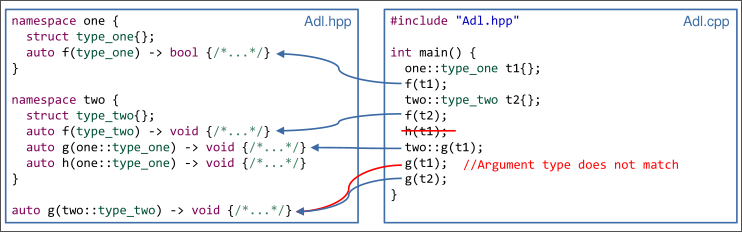
\includegraphics[scale=0.4]{2022-10-25-08:44:51.png}\newline
\textcolor{teal}{At the end, please do not rely too much on this, as it is not always clear what is being used}\\
\hline
Overwriting the std Namespace & 
\textcolor{orange}{Overwriting the standard namespace is not allowed!\newline
If you want to overwrite something in the std namespace use this workaround:}\newline
\begin{lstlisting}
using std::ostream;
using std::vector;
using out = std::ostream_iterator<int>;

namespace X { // create a namespace to use instead of the std vector
  struct vec : vector<int> { // vec is a new type
  using vector<int>::vector; // inherit ctors
};
// this is now allowed!!:
auto operator<<(ostream& os, vec const& v) -> ostream& { 
  copy(begin(v), end(v), out{os, ","});
  return os;
}
}
auto print(ostream& os) -> void {
  // copy all vector members to ostream and print them!
  using outv = std::ostream_iterator<X::vec>;
  vector<X::vec> vv{{1, 2, 3}, {4, 5, 6}};
  copy(begin(vv), end(vv), outv{os, "\n"});
}
\end{lstlisting}\\
\hline
\end{tabular}
\section{Enums}
\begin{tabular}{|m{0.2\linewidth}|m{0.755\linewidth}|}
\hline
Scopend and Unscoped Enums &
\textcolor{orange}{The difference is only the use of scope and the cast.}\newline
\begin{lstlisting}
// unscoped:
enum Day { 
  Mon, Tue, Wed, Thu, Fri, Sat, Sun
}; // 0, 1, 2, 3, 4, 5, 6
// conversion to int:
int day = Sun; // ok

// scoped:
enum class Day { 
  Mon, Tue, Wed, Thu, Fri, Sat, Sun
}; // 0, 1, 2, 3, 4, 5, 6
// conversion to int:
int day = Sun; // ERROR!
int day = static_cast<int>(Day::Sun); // ok

// Note, the scoped enum always requires the scope operator
auto test(Day day) {
  if (day == Day::Sun) { // scope used here, no scope for the regular enum!
    return true;
  }
  return false;
}
\end{lstlisting}\\
\hline
Int to Enum & 
\textcolor{orange}{Converting from int to enum always needs a cast:}\newline
\begin{lstlisting}
DayOfWeek tuesday = static_cast<DayOfWeek>(1);
\end{lstlisting}\\
\hline
Values for Enums &
\textcolor{teal}{You can specify the number for each part of an enum}\newline
\begin{lstlisting}
enum FilePermissions {
  readable = 1,  //001
  writeable = 2, //010
  executable = 4 //100
};
\end{lstlisting}\\
\hline

\hline

\hline

\hline

\hline
\end{tabular}
\end{table}
\pagebreak
\begin{table}[ht!]
\begin{tabular}{|m{0.2\linewidth}|m{0.755\linewidth}|}
\hline
Specifying Types & 
\textcolor{orange}{You can specify a type for an enum to use:}\newline
\begin{lstlisting}
enum LaunchPolicy : unsigned char {
sync = 1,
async = 2,
gpu = 4
}
\end{lstlisting} 
\, \newline
\textcolor{teal}{\textbf{Keep in mind that it will still have to be an integral type!!}}\\
\hline
Enum Operator Overloading & 
\begin{lstlisting}
enum DayOfWeek {
  Mon, Tue, Wed, Thu, Fri, Sat, Sun
};
auto operator++(DayOfWeek& aday) -> DayOfWeek {
  int day = (aday + 1) % (Sun + 1);
  aday = static_cast<DayOfWeek>(day);
  return aday;
}
\end{lstlisting}\\
\hline
\end{tabular}
\section{Containers}
\begin{tabular}{|m{0.2\linewidth}|m{0.755\linewidth}|}
\hline
Categories &
\vspace{2mm}
\begin{itemize}
\item \textcolor{orange}{Sequence Containers: \newline
  Elements are accessible in order as they were inserted/created\newline
  find in linear time through algorithm find}
\item \textcolor{orange}{Associative Containers:\newline
  Elements are accessible in sorted order\newline
  find as member function in logrithmic time}
\item \textcolor{orange}{Hashed Container (Unsorted Associative Container)\newline
  Element are accessible in unspecified order\newline
  find as member function in constant time}
\vspace{2mm}
\end{itemize}\\ 
\hline
General Container Info &
\vspace{2mm}
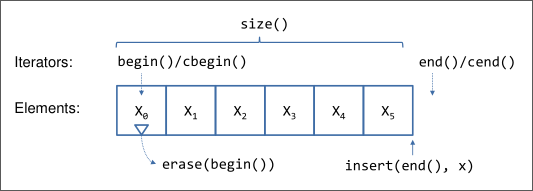
\includegraphics[scale=0.4]{2022-11-08-08:23:10.png}\newline
\begin{itemize}
\item \textcolor{orange}{begin()/end()}: Get iterators for algorithms and iteration in general
\item \textcolor{orange}{erase(iter)}: Removes the element at position the iterator iter points to
\item \textcolor{orange}{insert(iter, value)}: Inserts value at the position the iterator iter points to
\item \textcolor{orange}{size()/empty()}: Check the size of the container
\vspace{2mm}
\end{itemize}
\, \newline
\textcolor{teal}{Containers can be:}\newline
\begin{itemize}
  \item \textcolor{teal}{default-constructed}: std::vector<int> v{}
  \item \textcolor{teal}{copy-constructed}: std::vector<int> v2{v};
\item \textcolor{teal}{Equality compared if the same type}: if(v == v2)
\item \textcolor{teal}{lexicographically compared if elements can be compared}
\item \textcolor{teal}{emptied with clear()}
\vspace{2mm}
\end{itemize}\\
\hline
Initialization & 
\textcolor{orange}{Just like vectors, containers can usually be initialized via the 3 main methods: }\newline
\begin{itemize}
  \item \textcolor{teal}{initializer list}: std::vector<int> v{1,2,3,5,6};
  \item \textcolor{teal}{Construction with number of elements}: std::vector<int> v(5, 10);
  \item \textcolor{teal}{With range}: std::vector<int> v{cbegin(v), cend(v)};
\item \textcolor{teal}{item 4}
\vspace{2mm}
\end{itemize}\\
\hline
Sequence Containers & 
\vspace{2mm}
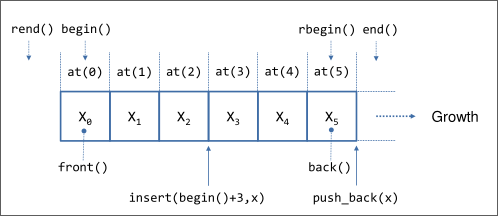
\includegraphics[scale=0.4]{2022-11-08-08:32:12.png}\newline
\begin{itemize}
\item \textcolor{teal}{std::vector}
\item \textcolor{teal}{std::deque}
\item \textcolor{teal}{std::list}
\item \textcolor{teal}{std::array}
\vspace{2mm}
\end{itemize}\\
\hline
std::array &
\vspace{2mm}
\begin{lstlisting}
std::array values{1,2,3,5,6};
// instead of
int obsolete[]{2,3,4,5,6};
\end{lstlisting}
\, \newline
\begin{itemize}
\item \textcolor{orange}{Fixed-size container, can't insert/append}
\item \textcolor{orange}{Can be initialized at compile time}
\item \textcolor{orange}{use std::array over C style array}
\item \textcolor{orange}{item 4}
\vspace{2mm}
\end{itemize}\\ 
\hline
\end{tabular}
\end{table}
\pagebreak
\begin{table}[ht!]
\begin{tabular}{|m{0.2\linewidth}|m{0.755\linewidth}|}
\hline
Double Ended queue std::deque & 
\vspace{2mm}
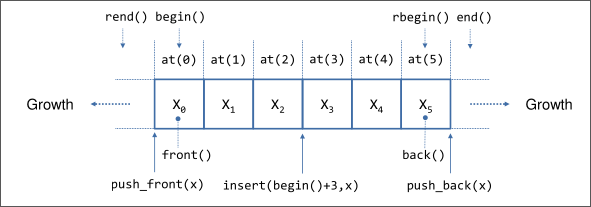
\includegraphics[scale=0.4]{2022-11-08-08:39:23.png}\newline
\textcolor{orange}{This is like the std::vector with the additional functions: \textbf{push\_front() and pop\_front()}}\newline
\textcolor{teal}{Special implementation for std::vector<bool> and std::deque<bool>.}\\
\hline
std::list & 
\vspace{2mm}
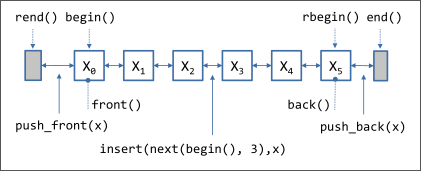
\includegraphics[scale=0.4]{2022-11-08-08:41:00.png}\newline
\begin{itemize}
\item \textcolor{orange}{Efficient insertion in any position}
\item \textcolor{orange}{Lower efficiency in bulk operations}
\item \textcolor{orange}{Requires member-function call for sort() etc}
\item \textcolor{orange}{Only bi-directional iterators - no index access!}
\vspace{-2mm}
\end{itemize}\\
\hline
std::forward\_list & 
\begin{lstlisting}
std::forward_list<int> l{1, 2, 3, 4, 5, 6};
\end{lstlisting}
\, \newline
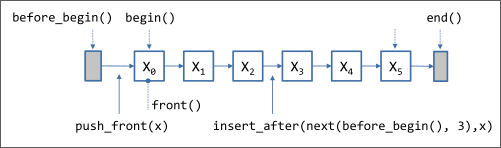
\includegraphics[scale=0.4]{2022-11-08-08:43:38.png}\newline
\begin{itemize}
\item \textcolor{orange}{Efficient insertion AFTER any position, but clumsy with iterator to get "before position"}
\item \textcolor{orange}{Only forward-iterators, lumsy to search and remove, use member-functions not algorithms}
\item \textcolor{orange}{Avoid, except when there is a specific need! \textbf{Better use std::list or std::vector}}
\vspace{-2mm}
\end{itemize}\\
\hline
std::stack & 
\begin{lstlisting}
std::stack<int> s{};
s.push(42);
std::cout << s.top();
s.pop();
\end{lstlisting}
\, \newline
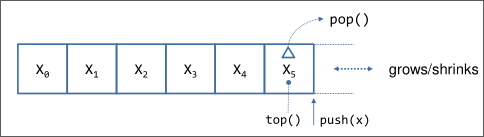
\includegraphics[scale=0.4]{2022-11-08-08:47:04.png}\newline
\begin{itemize}
\item \textcolor{orange}{Uses std::deque or std::vector/std::list and limits its functionality to stack operation}
\item \textcolor{orange}{No iteration}
\item \textcolor{orange}{Delegates push\_back(), back() and pop\_back()}
\item \textcolor{orange}{No longer a proper container, \textbf{deliberate limitation!}}
\vspace{-2mm}
\end{itemize}\\
\hline
std::queue & 
\begin{lstlisting}
std::queue<int> q{};
q.push(42);
std::cout << q.front();
q.pop();
\end{lstlisting}
\, \newline
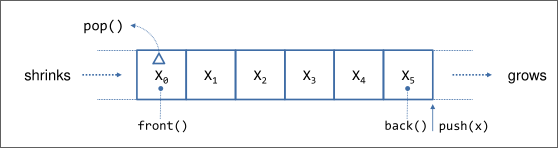
\includegraphics[scale=0.4]{2022-11-08-08:48:42.png}\newline
\begin{itemize}
\item \textcolor{orange}{Uses std::deque or std::vector/std::list and limits its functionality to stack operation}
\item \textcolor{orange}{No iteration}
\item \textcolor{orange}{Delegates push\_back(), back() and pop\_back()}
\item \textcolor{orange}{No longer a proper container, \textbf{deliberate limitation!}}
\vspace{-2mm}
\end{itemize}\\
\hline
std::priority\_queue & 
\begin{lstlisting}
std::priority_queue<int> q{};
q.push(42);
std::cout << q.front();
q.pop();
\end{lstlisting}
\, \newline
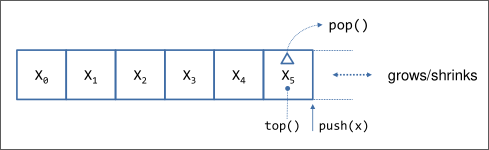
\includegraphics[scale=0.4]{2022-11-08-08:51:40.png}\newline
\begin{itemize}
\item \textcolor{orange}{Uses std::deque or std::vector/std::list and limits its functionality to stack operation}
\item \textcolor{orange}{No iteration}
\item \textcolor{orange}{Delegates push\_back(), back() and pop\_back()}
\item \textcolor{orange}{No longer a proper container, \textbf{deliberate limitation!}}
\item \textcolor{orange}{Keeps elements sorted}
\item \textcolor{orange}{top() element is always the smallest (requires elment type to be comparable)}
\vspace{-2mm}
\end{itemize}\\
\hline
\end{tabular}
\end{table}
\pagebreak
\begin{table}[ht!]
\begin{tabular}{|m{0.2\linewidth}|m{0.755\linewidth}|}
\hline
\vspace{2mm}
Associative Containers & 
\begin{itemize}
\item \textcolor{Orange}{Key Unique / Key only: std::set}
\item \textcolor{Orange}{Key Unique / Key and value: std::map}
\item \textcolor{Orange}{Multiple Equivalent Keys / Key only: std::multiset}
\item \textcolor{Orange}{Multiple Equivalent Keys / Key and value: std::multimap}
\vspace{-2mm}
\end{itemize}\\ 
\hline
std::set &
\begin{lstlisting}
std::set<int> values{5,6,2,9,8};
\end{lstlisting}
\, \newline
\begin{itemize}
\item \textcolor{orange}{Stores elements in sorted order (\textbf{ascending by default})}\newline
  order can be overwritten by the 2nd template parameter
\item \textcolor{orange}{Iteration walks over the elements in order}\newline
  Keys cannot be modified through iterators!
\item \textcolor{orange}{Use member functions for .find and .count}\newline
  Tree-search instead of sequential search\newline
  Result of .count(element is either 0 or 1\newline
  Since C++20 there is a .contains(element) member
\item \textcolor{orange}{Initializer does not need to be sorted}\newline
  s.contains(x) as quick check if x is present in std::set
\item \textcolor{orange}{Discouraged alternatives: s.find(x) != s.end() or s.count(x)}
\vspace{-2mm}
\end{itemize} 
\textcolor{orange}{Example:}\newline
\begin{lstlisting}
#include <iostream>
#include <set>
auto filterVowels(std::istream& in, std::ostream& out) -> void {
  std::set const vowels{'a', 'e', 'o', 'u', 'i', 'y'};
  char c{};
  while (in >> c) {
    if (!vowels.contains(c)) {
      out << c;
    }
  }
}
auto main() -> int {
  filterVowels(std::cin, std::cout);
}
\end{lstlisting}\\
\hline
std::map  &
\begin{lstlisting}
std::map<char, size_t> vowels{{'a', 3}, {'e', 8}, {'i', 5}, {'o', 4}, {'u', 2}, {'y', 1}};
\end{lstlisting}
\, \newline
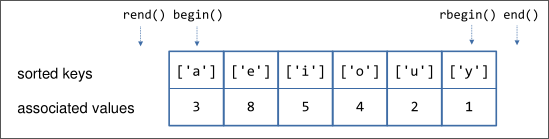
\includegraphics[scale=0.4]{2022-11-08-09:15:15.png}\newline
\begin{itemize}
\item \textcolor{Orange}{Stores key-value pairs in sorted order}\newline
  Sorted by key in ascending order\newline
  \textcolor{teal}{Order can be overwritten by the 3rd template parameter}
\item \textcolor{Orange}{Iterators access std::pair<key, value>}\newline
  Use .first for key and .second for value
\item \textcolor{orange}{m.contains(x) as quick check if x is a key present in std::map}\newline
  Discouraged alternative m.find(x) != m.end() or m.count(x)
\item \textcolor{orange}{auto is simpler than std::pair<key, value>, obviously lol}
\item \textcolor{orange}{Indexing operator[] inserts a new entry automatically if key is not present}\newline
  Key is the argument of the index operator, values is the default value of the value type\newline
  Returns the value by reference, which allows modification
\vspace{-2mm}
\end{itemize} 
\, \newline
\textcolor{orange}{Example:}\newline
\begin{lstlisting}
auto countVowels(std::istream& in, std::ostream& out) -> void {
  std::map<char, size_t> vowels{{'a', 0}, {'e', 0}, {'i', 0}, {'o', 0}, {'u', 0}, {'y', 0}};
  char c{};
  while (in >> c) {
    if (vowels.contains(c)) { // only count those chars that are already in the map
    ++vowels[c];
    for_each(cbegin(vowels), cend(vowels), [&out](auto const& entry) {
      // entry is a pair<char, size_t>
      out << entry.first << " = "<< entry.second << '\n';
    });
  }
}
\end{lstlisting}\\
\hline
std::multiset and std::multimap & 
\begin{lstlisting}
std::multiset<char> letters{'a', 'a', 'c', 'c', 'c', 'e', 'e', 'f'};
// note the c that appears 3 times!
\end{lstlisting}
\, \newline
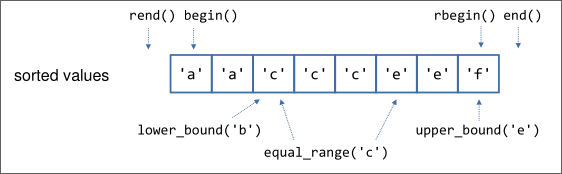
\includegraphics[scale=0.4]{2022-11-08-09:24:23.png}\newline
\begin{itemize}
\item \textcolor{orange}{Multiple Keys allowed}\newline
  Use equal\_range() or lower\_bound()/upper\_bound() member functions/algorithms to find boundaries of equivalent keys
\item \textcolor{orange}{Can be a bit more tedious to work with than std::set}
\vspace{-2mm}
\end{itemize} \\
\hline
\end{tabular}
\end{table}
\pagebreak
\begin{table}[ht!]
\begin{tabular}{|m{0.2\linewidth}|m{0.755\linewidth}|}
\hline
&
\textcolor{orange}{Example:}\newline
\begin{lstlisting}
auto sortedStringList(std::istream& in, std::ostream& out) -> void {
  using inIter = std::istream_iterator<std::string>;
  using outIter = std::ostream_iterator<std::string>;
  std::multiset<std::string> words{inIter{in}, inIter{}};
  copy(cbegin(words), cend(words), outIter(out, "\n"));
  auto current = cbegin(words);
  while (current != cend(words)) {
    auto endOfRange = words.upper_bound(*current);
    copy(current, endOfRange, outIter{out, ", "});
    out << '\n'; // next range on new line
    current = endOfRange;
  }
}
\end{lstlisting} 
\begin{itemize}
\item \textcolor{orange}{First copy-algorithm call prints each word on separate line}
\item \textcolor{orange}{Code in while-loop groups equivalent words on one line}
\vspace{-2mm}
\end{itemize} \\
\hline
std::unordered\_set & 
\begin{lstlisting}
#include <algorithm>
#include <iostream>
#include <iterator>
#include <unordered_set>
auto main() -> int {
  std::unordered_set<char> const vowels{'a', 'e', 'i', 'o', 'u'};
  using in = std::istreambuf_iterator<char>;
  using out = std::ostreambuf_iterator<char>;
  remove_copy_if(in{std::cin}, in{}, out{std::cout},
  [&](char c) { return vowels.count(c); }
  );
}
\end{lstlisting}
\, \newline
\begin{itemize}
\item \textcolor{orange}{Usage is almost equivalent to std::map}\newline
  Except lack of ordering
\item \textcolor{orange}{Don't use std::unordered\_map with your own types, unless you are an expert in hash functions and you benefit from the speedup}\newline
  Boost library provides hash-combiner helper
\vspace{-2mm}
\end{itemize} \\
\hline
std::unordered\_map & 
\begin{lstlisting}
#include <iostream>
#include <string>
#include <unordered_map>
auto main() -> int {
  std::unordered_map<std::string, int> words{};
  std::string s{};
  while (std::cin >> s) { ++words[s]; }
    for(auto const& p : words) {
    std::cout << p.first << " = "<< p.second << '\n';
  }
}
\end{lstlisting}
\, \newline
\begin{itemize}
\item \textcolor{orange}{Usage is almost equivalent to std::map}\newline
  Except lack of ordering
\item \textcolor{orange}{Don't use std::unordered\_map with your own types, unless you are an expert in hash functions and you benefit from the speedup}\newline
  Boost library provides hash-combiner helper
\vspace{-2mm}
\end{itemize} \\
\hline
\end{tabular}
\section{Iterators}
\begin{tabular}{|m{0.2\linewidth}|m{0.755\linewidth}|}
\hline
Different Iterators & 
\textcolor{orange}{There are 2 different main categories, input iterators and output iterators.\newline
The input iterators has a bunch of parent-iterators with different behaviors}\newline
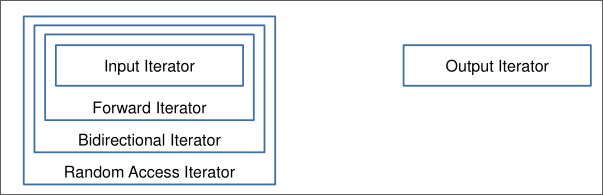
\includegraphics[scale=0.4]{2022-11-08-09:34:02.png}\newline
\textcolor{teal}{The more you move outwards on the input iterator, the more power these iterators have!}\\
\hline
Input Iterators & 
\begin{lstlisting}
struct input_iterator_tag{};
auto operator* () -> Element;
auto operator++() -> It&;
auto operator++(int) -> It;
auto operator==(It const&) -> bool;
auto operator!=(It const&) -> bool;
auto operator= (It const&) -> It&;
It(It const&); //copy ctor
\end{lstlisting} 
\, \newline
\begin{itemize}
\item \textcolor{orange}{Supports reading the "current" element}
\item \textcolor{orange}{Allows for one-pass input algorithms}\newline
  \textcolor{red}{Can't step backwards}
\item \textcolor{orange}{Models the std::istream\_iterator and std::istream}
\item \textcolor{orange}{Can be compared with == and !=}\newline
  To other iterator objects of teh sae type: It
\item \textcolor{orange}{Can be copied}\newline
  \textcolor{red}{After increment (calling ++) all other copies are invalid!}\newline
  *it++ is allowed explicitly (by the standard)
\vspace{-2mm}
\end{itemize}\\
\hline
\end{tabular}
\end{table}
\pagebreak
\begin{table}[ht!]
\begin{tabular}{|m{0.2\linewidth}|m{0.755\linewidth}|}
\hline
Forward Iterators &
\begin{lstlisting}
struct forward_iterator_tag{};
auto operator* () -> Element&;
auto operator++() -> It&;
auto operator++(int) -> It;
auto operator==(It const&) -> bool;
auto operator!=(It const&) -> bool;
auto operator= (It const&) -> It&;
It(It const&); //copy ctor
\end{lstlisting} 
\, \newline
\begin{itemize}
\item \textcolor{orange}{Can do whatever an input iterator can do, and:} \newline
  \textcolor{teal}{Supports changing the "current" element, unless elements are const}
\item \textcolor{orange}{Still allows only for one-pass input algorithms}\newline
  \textcolor{red}{Can't step backwards}\newline
  But can keep iterator copy around for later reference
\item \textcolor{orange}{Models the std::forward\_list iterators}
\vspace{-2mm}
\end{itemize} \\
\hline
Bidirectional Iterator & 
\begin{lstlisting}
struct bidirectional_iterator_tag{};
auto operator* () -> Element&;
auto operator++() -> It&;
auto operator++(int) -> It;
auto operator--() -> It&;
auto operator--(int) -> It;
auto operator==(It const&) -> bool;
auto operator!=(It const&) -> bool;
auto operator= (It const&) -> It&;
It(It const&); //copy ctor
\end{lstlisting}
\, \newline
\begin{itemize}
\item \textcolor{orange}{Can do whatever a forward iterator can, plus..}\newline
  \textcolor{red}{CAN GO BACKWARDS}
\item \textcolor{orange}{Allows for forward-backwards-pass algorithms}
\item \textcolor{orange}{Models the std::iterators}
\vspace{-2mm}
\end{itemize}\\ 
\hline
Random Access Iterators & 
\begin{lstlisting}
struct random_access_iterator_tag{};

auto operator* () -> Element&;
auto operator++() -> It&;
auto operator++(int) -> It;
auto operator--() -> It&;
auto operator--(int) -> It;
auto operator==(It const&) -> bool;
auto operator!=(It const&) -> bool;
auto operator= (It const&) -> It&;
It(It const&); //copy ctor
auto operator[](distance) -> Element&;
auto operator+(distance) -> It;
auto operator+=(distance) -> It&;
auto operator-(distance) -> It;
auto operator-=(distance) -> It&;
auto operator-(It const &) -> distance;
//relational operators, like <
\end{lstlisting}
\, \newline
\begin{itemize}
\item \textcolor{orange}{Can do whatever a bidirectional iterator can, plus..}\newline
  \begin{itemize}
  \item \textcolor{teal}{Directly access element at index (offset to current position): distance can be positive or negative}
  \item \textcolor{teal}{Go n steps forward or backwards}
  \item \textcolor{teal}{"Subtact" two iterators to get the distance}
  \item \textcolor{teal}{Compare with relational operators (<, <=, >, >=)}
  \end{itemize} 
\item \textcolor{orange}{Allows random access in algorithms}
\item \textcolor{orange}{Models the std::vector iterators}
\vspace{-2mm}
\end{itemize} \\
\hline
\end{tabular}
\end{table}
\pagebreak
\begin{table}[ht!]
\begin{tabular}{|m{0.2\linewidth}|m{0.755\linewidth}|}
\hline
Output Iterator & 
\begin{lstlisting}
struct output_iterator_tag{};
auto operator*() -> Element&;
auto operator++() -> It&;
auto operator++(int) -> It;
\end{lstlisting}
\, \newline
\begin{itemize}
\item \textcolor{orange}{Can write value to current element, but only once (*it = value)}\newline
  Then increment is required
\item \textcolor{orange}{Modeled after std::ostream\_iterator}
\item \textcolor{orange}{Most other iterators can also act as output iterators}\newline
  \textcolor{red}{Unless the underlying container is const}
\item \textcolor{orange}{Exception: associative containers will allow only read-only iteration}
\item \textcolor{orange}{No comparison and end to an out rang is not queryable}
\vspace{-2mm}
\end{itemize}\\ 
\hline
std::distance(start, goal) & 
\begin{itemize}
  \item \textcolor{orange}{counts the number of hops it needs to take to the goal}  
\item \textcolor{orange}{Efficient for random access iterators}
\item \textcolor{orange}{For other iterators it has to loop -> not efficient}\newline
  This also implies that the goal has to be after start.
\vspace{-2mm}
\end{itemize}\\ 
\hline
std::advance(itr, n) & 
\textcolor{orange}{std::advance simply moves x steps forward or backwards ( if the iterator allows it!)}\newline
\begin{itemize}
\item \textcolor{teal}{Efficient for random access iterators}
\item \textcolor{teal}{returns void -> no copies made}
\vspace{-2mm}
\end{itemize} \\
\hline
std::next() / std::prev() & 
\textcolor{orange}{Goes one step further/back on the iterator and returns a copy of the value in the container at the next index.}\newline
\textcolor{teal}{The step can be specified to be something other than 1 with a temporary argument!}\\
\hline
const iterators & 
\textcolor{red}{A const iterator does not mean that the iterator itself is const, only the elements behind it are! In other words, it just doesn't allow you to modify the elements behind it.}\newline
\begin{lstlisting}
std::vector v{3, 1, 4, 1, 5, 9, 2, 6};
auto const iter1 = values.begin(); //std::vector<int>::iterator const
++iter1;
auto iter2 = values.cbegin(); //std::vector<int>::const_iterator
*iter = 2;
\end{lstlisting}
\, \newline
\textcolor{teal}{Here we would try to change the value behind the iterator, this doesn't work with const iterators!}\\
\hline
\end{tabular}
\section{Algorithms}
\begin{tabular}{|m{0.2\linewidth}|m{0.755\linewidth}|}
\hline 
Different Algorithms and numberic functions & 
\minipg{
Algorithms:\newline
\begin{itemize}
\item \textcolor{purple}{Filling}
\item \textcolor{purple}{Finding}
\item \textcolor{purple}{Property checking}
\item \textcolor{purple}{Transformation}
\end{itemize} 
}{
Numerics:\newline
\begin{itemize}
\item \textcolor{purple}{Generic numberic functions}
\item \textcolor{purple}{Some functions can be applied in on numeric contexts}
\end{itemize} 
}[0.4,0.4]\\
\hline
Why? & 
Why do we use algorithms over loops and other code?\newline
It is very simple, \textbf{algorithms are easy and safe to use without x amount of possibilities for errors!}\newline
Think about a loop, you need to make sure you are in the bounds of the vector, or that you assign the right value at each time...\newline
With algorithms we just say here is range go do stuff.
Reasons for algorithms:\newline
\begin{itemize}
\item \textcolor{purple}{Correctness}\newline
  Handwritten algorithms are often error prone and need time debugging!
\item \textcolor{purple}{Readability}\newline
  Handwritten algorithms are often conveluted and need lots of time reading and understanding.
\item \textcolor{purple}{Performance}\newline
  Unless you are very good at what you do, the standard algorithms are likely faster!
\vspace{-3mm}
\end{itemize} 
\\
\hline
for\_each & 
For loop using 2 iterators -> \textbf{begin()} and \textbf{end()} as well as a \textbf{lambda} as the function to execute on each element.\newline
\begin{lstlisting}
auto values = std::vector{3, 0, 1, 4, 0, 2};
auto f = [](auto v) {};
std::for_each(begin(values), end(values), f);
\end{lstlisting}\\
\hline
Functors & 
Functors are just overloaded structs or classes on the () operator.\newline
\textbf{As expected, you can then use this struct or class like it is a function!}\newline
Here is how to implement it:\newline 
\begin{lstlisting}
struct Accumulator {
  int count{0};
  int accumulatedValue{0};
  auto operator()(int value) -> void {
    count++;
    accumulatedValue += value;
  }
  int average() const;
  int sum() const;
};
auto average(std::vector<int> values) -> int {
  Accumulator acc{};
  for(auto v : values) { acc(v); }
  return acc.average();
}

auto average(std::vector<int> values) -> int {
  auto acc = Accumulator{};
  return std::for_each(begin(values), end(values), acc).average();
}
\end{lstlisting}\\
\hline
\end{tabular}
\end{table}
\pagebreak
\begin{table}[ht!]
\begin{tabular}{|m{0.2\linewidth}|m{0.755\linewidth}|}
\hline
Additional Argument to Associative Containers & 
You can pass a bool lambda to associative containers, this means that the result of the predicate must be false or true.\newline
The idea is that you can give a sorting algorithm to the set in order to easily sort it out of the box.\newline
\begin{lstlisting}
std::set<int, std::greater<>> reverse_int_set{};
\end{lstlisting}
\textcolor{OliveGreen}{Note that this lambda must be \textbf{transitive and irreflexive}}\newline
Transitive: \(x > y\) and \(y > z\), then also \(x > z\)\newline
Irreflexive: \\
\hline
Transform & 
Transform uses 2 vectors with a lambda to perform a function on each element in both vectors.\newline
\begin{lstlisting}
auto counts = std::vector{3, 0, 1, 4, 0, 2};
auto letters = std::vector{'g', 'a', 'u', 'y', 'f', 'o'};
auto combined = std::vector<std::string>{};
auto times = [](auto i, auto c) { return std::string(i, c); };
std::transform(begin(counts), end(counts), begin(letters),
std::back_inserter(combined), times);
\end{lstlisting}
Here we would print each character x amount of times, with x being the same index element in the counts vector.\\
\hline
Merge & 
Mergesort takes 2 sorted vectors and puts them together:\newline
\begin{lstlisting}
std::vector r1{9, 12, 17, 23, 54, 57, 85, 95};
std::vector r2{2, 30, 32, 41, 49, 63, 72, 88};
std::vector d(r1.size() + r2.size(), 0);
std::merge(begin(r1), end(r1), begin(r2), end(r2), begin(d));
// 2,9,12,17,23,30,32,41,49,54,57,63,72,85,88,95
\end{lstlisting}\\
\hline
Remove and Erase & 
\textcolor{red}{Remove will not actually \textbf{remove} the elements, instead, it will mark them as removable in order to not cause iterator invalidation!}\newline
\textcolor{OliveGreen}{If you want to properly remove them, then you can also call erase which will then free the marked elements!}\newline
\begin{lstlisting}
auto values = std::vector{54, 13, 17, 95, 2, 57, 12, 9};
auto is_prime = [](unsigned u) { u > 20};
auto removed = std::remove_if(begin(values), end(values), is_prime);
// mark 2,9,12,13,17 as to remove
values.erase(removed, values.end());
// erase the marked elements
// vector is now -> 54,57,95
\end{lstlisting} 
remove\_if just has an additional boolean check which can be done with a lambda, use case is shown here for filtering!\\
\hline
Accumulate & 
Sum function:\newline
\begin{lstlisting}
std::vector<std::string> longMonths{"Jan", "Mar", "May", "Jul", "Aug", "Oct", "Dec"};
auto accumulatedString = std::accumulate(
next(begin(longMonths)), //Second element
end(longMonths),
//End
longMonths.at(0),
//First element, usually the neutral element
[](std::string const & acc, std::string const & element) {
return acc + ", " + element;
}); //Jan, Mar, May, Jul, Aug, Oct, Dec
\end{lstlisting}\\
\hline
\_if suffix & 
Just like the remove\_if, there are many other algorithms that implement the if keyword to \textbf{only execute this algorithm when the boolean check is true}.\newline
Often they are used in combination with \textbf{lambdas}!
\begin{lstlisting}
auto numbers = std::set{1, 2, 3, 4, 5, 6, 7, 8, 9};
auto isPrime = [](auto u) {/*...*/};
auto nOfPrimes = std::count_if(begin(numbers), end(numbers), isPrime);
\end{lstlisting}
\, \newline
List of Algorithms with the if suffix:\newline
\minipg{
\begin{itemize}
\item \textcolor{teal}{count\_if}
\item \textcolor{teal}{find\_if}
\item \textcolor{teal}{find\_if\_not}
\item \textcolor{teal}{copy\_if}
\end{itemize} 
}{\begin{itemize}
\item \textcolor{teal}{count\_if}
\item \textcolor{teal}{find\_if}
\item \textcolor{teal}{find\_if\_not}
\item \textcolor{teal}{copy\_if}
\end{itemize} 
}[0.4,0.4]\\
\hline
Algorithms \_n Versions & 
Instead of always going through the entire list, you can also use the \_n suffix algorithms to specify a different endpoint for this algorithm, for example in a vector with 7 elements you might want to only do the first 5 elements, therefore the additional parameter will be 5, for 5 elements!\newline
\begin{lstlisting}
auto numbers = std::set{1, 2, 3, 4, 5, 6, 7, 8, 9};
auto top5 = std::vector<int>(5);
std::copy_n(rbegin(numbers), 5, begin(top5));
\end{lstlisting}
\, \newline
\begin{itemize}
\item \textcolor{teal}{search\_n}
\item \textcolor{teal}{copy\_n}
\item \textcolor{teal}{fill\_n}
\item \textcolor{teal}{generate\_n}
\item \textcolor{teal}{for\_each\_n}
\vspace{-3mm}
\end{itemize}\\ 
\hline
Heap Algorithm & 
\begin{lstlisting}
std::vector<int> v{3,1,4,1,5,9,2,6};
make_heap(v.begin(),v.end());
pop_heap(v.begin(),v.end());
v.pop_back();
v.push_back(8);
push_heap(v.begin(),v.end());
sort_heap(v.begin(),v.end());
\end{lstlisting}\\
\hline
Don't mixmatch Iterators & 
\textcolor{red}{Don't mixmatch iterators!}:\newline
\begin{lstlisting}
std::vector<unsigned> values1 = create_vector();
std::vector<unsigned> values2 = create_vector();
auto f = [](unsigned u) {/*...*/};
std::for_each(begin(values1), end(values2), f);
\end{lstlisting}
\\
\hline
\end{tabular}
\end{table}
\pagebreak
\begin{table}[ht!]
\begin{tabular}{|m{0.2\linewidth}|m{0.755\linewidth}|}
\hline
Make sure that enough space is allocated in a vector & 
\textcolor{red}{Make sure that enough space is allocated for when you copy data!}\newline
\begin{lstlisting}
std::set<unsigned> numbers{1, 2, 3, 4, 5, 6, 7, 8, 9};
std::vector<unsigned> primes{};
auto isPrime = [](unsigned u) {/*...*/};
std::copy_if(begin(numbers), end(numbers), begin(primes), isPrime);
\end{lstlisting}
\, \newline
So how do we properly do this? \textbf{Inserters!}\newline
\begin{lstlisting}
std::set<unsigned> numbers{1, 2, 3, 4, 5, 6, 7, 8, 9};
std::vector<unsigned> primes{};
auto is_prime = [](unsigned u) {/*...*/};
std::copy_if(begin(numbers), end(numbers), back_inserter(primes), is_prime);
\end{lstlisting}
\, \newline
There are 3 such inserters:\newline
\begin{itemize}
\item \textcolor{purple}{back\_inserter}\newline
  uses the \textbf{push\_back function} to insert at the back
\item \textcolor{purple}{front\_inserter}\newline
  uses the \textbf{push\_front function} to insert at the front
\item \textcolor{purple}{inserter}\newline
  uses the \textbf{insert member} function to insert
\item \textcolor{purple}{item 4}
\vspace{-3mm}
\end{itemize} \\
\hline
Iterator invalidation & 
If you change a vectors size during an algorithm or a loop, you have the problem that your vector might change size. \newline
The side effect is that \textbf{your vector will resize!} This means that \textbf{it will move to another memory location!}\newline
Because of the new memory location \textbf{your iterators are now invalid!}\newline
Avoid modifying vector sizes during iteration, instead use the same system as the remove does, mark them and then modify the vector size later or create a new one.\\
\hline
Using ranges & 
You can of course also use ranges instead should they work with your compiler, lol :P\newline
\begin{lstlisting}
auto values = std::vector<int>{3, 1, 4, 1, 5, 9};
// old
std::reverse(begin(values), end(values));
// new
std::ranges::reverse(values);
\end{lstlisting}\\
\hline
Non-Modifying Algorithms & 
\vspace{2mm}
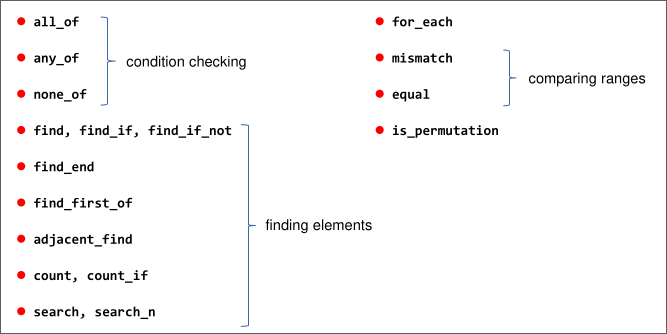
\includegraphics[scale=0.4]{2022-11-15-09:43:09.png}\\
\hline
Mutating Sequence Operations & 
\vspace{2mm}
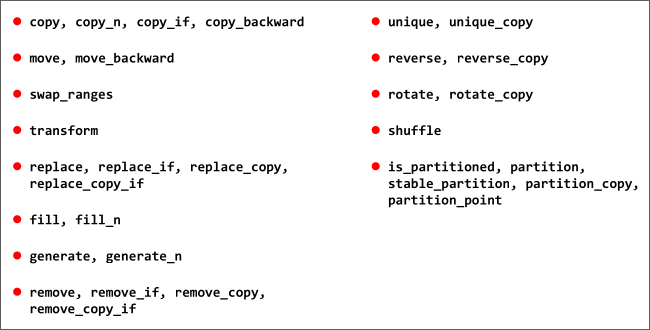
\includegraphics[scale=0.4]{2022-11-15-09:43:15.png}\\
\hline
Sorting Algorithms and Related Operations & 
\vspace{2mm}
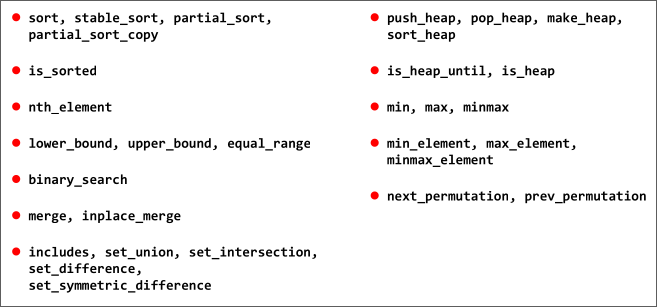
\includegraphics[scale=0.4]{2022-11-15-09:43:22.png}\\
\hline
\end{tabular}
\end{table}
\pagebreak
\begin{table}[ht!]
\section{Templates}
\begin{tabular}{|m{0.2\linewidth}|m{0.755\linewidth}|}
\hline
Basics & 
You can use one or more types to use in templates.\newline
\textcolor{OliveGreen}{Note that you usually write the template definition inside the header file!\newline
\textbf{This also means that templates are implicitly inline!!}}\newline
\begin{lstlisting}
template <typename T>
  auto min(T left, T right) -> T {
    return left < right ? left : right;
}
\end{lstlisting} 
For the writing in the header file part, the reason for this is that you could only use that template function inside of one cpp file. Usually this makes no sense so we define it in the header, this way we can export the function.\\
\hline
Compiler checks & 
The compiler checks the template code twice, the first time when it sees the template function itself, here it only does basic syntax checking, does the template make sense, are there any missing semicolons etc.\newline
The next time it checks is at instantiation, here it will do proper checking, like can this type actually be used in this function with all the operators that are used here?\\
\hline
Duck typing & 
"If it walks and quacks like a duck, it must be a duck"\newline
C++ has a similar way of doing generics as rust, it will simply do the operation if the type has said operation.\newline
In rust the same is guaranteed, the only difference is that the guarantee usually comes from a trait, while in c++ it must come from the type itself.\newline
With c++ 20 you can technically also do the same in c++ as you did in rust, but once again funny funny maybe worky maybe noty.\\
\hline
Type matching & 
The c++ compiler only does extremely exact matching, meaning a double and an int will not match to either double double or int int:\newline
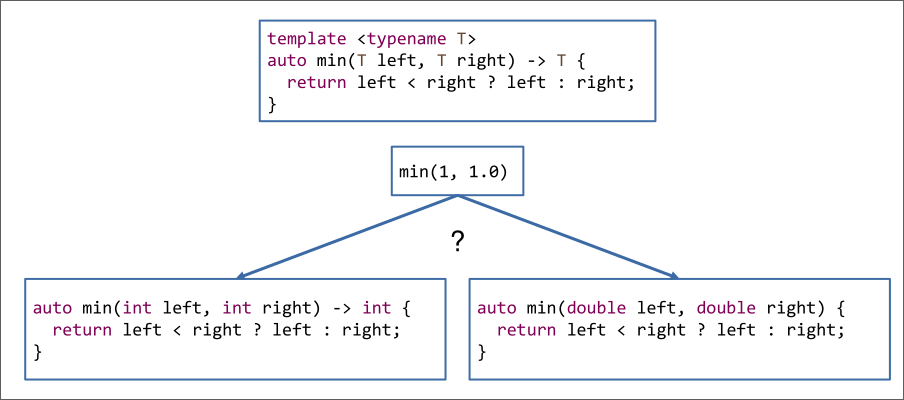
\includegraphics[scale=0.4]{2022-11-22-08:46:33.png}\\
\hline
Variable templates & 
C++ compiler allows for a variable number of templates which can then also be used in a function!\newline
\begin{lstlisting}
auto printAll() -> void {} // needed for printAll with the last case where first is empty!
template<typename First, typename...Types>
  auto printAll(First const & first, Types const &...rest) -> void {
  std::cout << first;
  if (sizeof...(Types)) {
    std::cout << ", ";
  }
  printAll(rest...);
  // print the variable numbers of parameters
}
\end{lstlisting}
\textcolor{OliveGreen}{Note that the variable number of types needs to be the last part of both the template and the parameter list!!}\\
\hline
Packing and unpacking & 
As you can see above and similar to rust, you can use the ... operator to indicate packing inside the template functions.\newline
Here it will put together the types with \textbf{Types const \&...rest} and then unpack to use again inside a function with \textbf{rest...}\newline
\textcolor{OliveGreen}{This is just syntax sugar, the code that will be generated will have hardcoded variables again, you just don't see them in c++ -> only in machine code!}\\
\hline
Template overloading & 
You can overload a template if you for example want to use pointers instead of the actual type, or you can even write an overload for an explicit type:\newline
\begin{lstlisting}
template <typename T>
  auto min(T left, T right) -> T {
    return left < right ? left : right;
}
template <typename T>
  auto * min(T * left, T * right) -> T {
    return *left < *right ? left : right;
}
auto min(char const * left, char const * right) -> char const * {
return std::string{left} < std::string{right} ? left : right;
}
\end{lstlisting}\\
\hline
Generic Operator functions &
You can create generic operator functions with either a struct or a lambda, but this might not always work, as there are often more specific matches which will be called instead!\newline
\begin{lstlisting}
// lambda
auto const printer = [&out](auto const & e) {
  out << "Element: " << e;
};

// struct method
struct __PrinterLambda {
  template <typename T>
  auto operator()(T const & e) const -> void {
    __out << "Element: " << e;
  }
  std::ostream & __out;
};
\end{lstlisting}\\
\hline
\end{tabular}
\end{table}
\pagebreak
\begin{table}[ht!]
\begin{tabular}{|m{0.2\linewidth}|m{0.755\linewidth}|}
\hline
Converting C string literals to c++ standard literals & 
C string literals are stored in a char array, this makes it hard to be used, as arrays don't have any special functions attached to them.\newline
We can instead use std::string\_literals to for example make printing work with string literals:\newline
\begin{lstlisting}
using namespace std::string_literals;
std::cout << min("C++"s, "Java"s);
\end{lstlisting}\\
\hline
More specificity problems & 
\begin{lstlisting}
template <typename T>
  auto min(T & left, T & right) -> T {
    return left < right ? left : right;
}
auto min(std::string const & left, std::string const & right) -> std::string {
  return std::ranges::lexicographical_compare(left, right, [](char l, char r) {
    return tolower(l) < tolower(r);
  }) ? left : right;
}
std::string small{"aa"};
std::string capital{"ZZ"};
std::cout << min(small, capital) << '\n'; //ZZ
\end{lstlisting}
Here the problem would be that we didn't specify the string as const, this mean the template would be called, which didn't specify that we want to compare the lower symbols only. Bigger symbols are always higher up in the ascii table, meaning we get the wrong behavior with ZZ being "smaller" than aa!\\
\hline
Dangling references or rather why to use rust & 
The following is exactly why borrowing just works, we pass 2 references to a function and receive the value of one of them. The problem is that the lifetime of the temporary reference of the parameters will be invalid after the semicolon, exactly like in rust!\newline
This means you could potentially be getting invalid values!\newline 
\begin{lstlisting}
template <typename T>
auto const & min(T const & left, T const & right) -> T {
return left < right ? left : right;
// left and right now dead as lifetime not extended
// in other words, return is invalid
}
std::string const & smaller = min("a"s, "b"s);
std::cout << "smaller is: " << smaller; // undefined behavior! might or might not work!
\end{lstlisting}
\textcolor{OliveGreen}{The fix is to return a const \& reference as well, as this would extend the lifetime of the reference!}\newline
\begin{lstlisting}
template <typename T>
auto min(T const & left, T const & right) -> T const & {
  return left < right ? left : right;
}
\end{lstlisting}\\
\hline
\end{tabular}
\section{Class Templates}
\begin{tabular}{|m{0.2\linewidth}|m{0.755\linewidth}|}
\hline
Basics & 
These are the same as before, just nested within a class to give you flexiblity to create a generic class. \newline
\begin{lstlisting}
template <typename T> class Sack {
  using SackType = std::vector<T>;
  // ATTENTION, typename needed here for size_type.
  using size_type = typename SackType::size_type;
  SackType theSack{};
public:
  auto empty() const -> bool {
    return theSack.empty();
  }
  auto size() const -> size_type{
    return theSack.size();
  }
  auto putInto(T const & item) -> void {
    theSack.push_back(item);
  }
  auto getOut() -> T; //Implementation out of line
};
\end{lstlisting}\\
\hline
Typedef vs using & 
Use using instead of typedef as it is newer and can do the following while typedef can't:\newline
\begin{lstlisting}
// ok
using someName = std::vector<T>;
// ERROR BRO
typedef std::vector<T> someName;
\end{lstlisting}\\
\hline
Typename for dependent names & 
Within the template definition you might use names that are directly or indirectly depending on the template parameter.\newline
This would mean an endless loop of dependency, to solve this we need to use typename.\newline
\begin{lstlisting}
// examples
template <typename T> void accessTsMembers() {
  typename T::MemberType m{};
  T::StaticMemberFunction();
  T::StaticMemberVariable;
}

template<typename T> class Sack {
  using size_type = typename std::vector<T>::size_type;
  //...
};
\end{lstlisting}\\
\hline
\end{tabular}
\end{table}
\pagebreak 
\begin{table}[ht!]
\begin{tabular}{|m{0.2\linewidth}|m{0.755\linewidth}|}
\hline
Static Member variables &
Static Member variables are \textbf{semi global variables with a double colon scope.}\newline
\textcolor{purple}{Global in the sense of each individual type has their own version of it. So if we override the variant for integers, then each integer will access the same value!}\newline
You can add static structs via inline like this: \newline
\begin{lstlisting}
template <typename T> struct StaticMember {
  inline static int member{sizeof(T)};
};
\end{lstlisting}
\, \newline
Here an example how you can use this: \newline
\begin{lstlisting}
// class.hpp
template <typename T> struct StaticMember {
  inline static int member{sizeof(T)};
};

// class.cpp
#include "staticMember.hpp"
auto setMemberTo42() -> int {
  using MemberType = StaticMember<int>;
  MemberType::member = 42;
  return MemberType::member;
}

// main.cpp
#include "staticMember.hpp"
#include <iostream>
auto setMemberTo42() -> int;
auto main() -> int {
  std::cout << StaticMember<double>::member << '\n'; // 8
  std::cout << StaticMember<int>::member << '\n';    // 4
  std::cout << setMemberTo42() << '\n'; // overrides!   42
  std::cout << StaticMember<int>::member << '\n';    // 42
}
\end{lstlisting}\\
\hline
Dependent names and specificity in template classes & 
For templates it is better to use the this keyword as otherwise you could potentially use another function that is not inside the class.\newline
To avoid this, you can add either double colons or the this keyword to avoid problems.\newline 
\begin{lstlisting}
template <typename T>
struct Parent {
  auto foo() const -> int { // can be called with this->foo()
  return 42;
  }
  static int const bar{43}; // accessed with this->bar
};
auto foo() -> int { // can be called with foo()
  return 1;
}
double const bar{3.14}; // accessed with bar
\end{lstlisting}\\
\hline
Containers with pointers & 
When we use pointers in containers, we have the problem that we can create containers with pointers inside them. \newline
As expected nobody will give us the guarantee that these pointers will still be valid at any given time.\newline
To solve this we can create a specific template that is more specific to pointer which makes sure we will not have this issue:\newline
\begin{lstlisting}
// Partial Specialization
template <typename T>
struct Sack<T *>;

// Explicit Specialization
template <>
struct Sack<char const *>;
\end{lstlisting} 
\, \newline
These can then be used to make sure that the values will still be valid.\newline
We can however, also just prevent the creation of point based containers:\newline
\begin{lstlisting}
template <typename T> struct Sack<T *> {
  ~Sack() = delete; // lmao delete constructor
};

// while the char const can be done with something like std::vector<string> instead
template <> struct Sack<char const *> {
  using SackType = std::vector<std::string>;
  using size_type = SackType::size_type;
  SackType theSack;
}
\end{lstlisting}\\
\hline
Type casting overload & 
In order to cast a type to another, you must overload the operator for this, or use another function instead:\newline
\begin{lstlisting}
// Overload 
template <typename Elt>
  explicit operator std::vector<Elt>() const {
    return std::vector<Elt>(begin(theSack), end(theSack));
}

// other function 
template <typename Elt = T>
  auto asVector() const {
  return std::vector<Elt>(begin(theSack), end(theSack));
}
\end{lstlisting}\\
\hline
\end{tabular}
\end{table}
\pagebreak 
\begin{table}[ht!]
\begin{tabular}{|m{0.2\linewidth}|m{0.755\linewidth}|}
\hline
Type deduction with structs & 
Since C++ 17 the compiler can deduce the typename that you have specified at the top when using functions from classes etc: \newline
\begin{lstlisting}
template <typename T> struct Box {
  Box(T content) : content{content}{}
  T content;
};
auto main() -> int {
  Box<int> b0{0}; //Before C++17
  Box      b1{1}; //Since C++17
}
\end{lstlisting} \\
\hline
Type deduction with initializer lists & 
Initializer list allow us to create a container without specifiying the type, as it is implicitly passed by the values that you enter:\newline
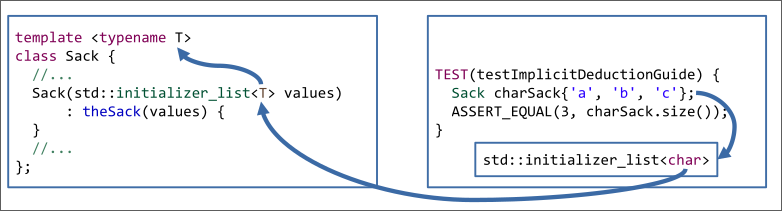
\includegraphics[scale=0.4]{2022-11-29-09:27:18.png}\\
\hline
Type deduction with Iterators & 
When we want to use type deduction with iterators, then we need a way to do this with iterators.\newline
Obviously this is not done out of the box, therefore we need another way to do this: \newline
\begin{lstlisting}
template <typename Iter>
Sack(Iter begin, Iter end) -> Sack<typename std::iterator_traits<Iter>::value_type>;

TEST(testDeductionForIterators) {
  std::vector values{3, 1, 4, 1, 5, 9, 2, 6};
  Sack aSack(begin(values), end(values));
  ASSERT_EQUAL(values.size(), aSack.size());
}
// Note without the template above, aSack would not compile!
\end{lstlisting}\\
\hline
Passing a standard container as template parameter & 
Sometimes we want to have a container itself as a template container, which will be used instead of one harcoded variant.\newline
\begin{lstlisting}
Sack<unsigned, std::set> aSack{1, 2, 3};

auto getOut() -> T {
  throwIfEmpty();
  auto index = static_cast<size_type>(rand() % size());
  auto it = begin(theSack);
  advance(it, index);
  T retval{*it};
  theSack.erase(it);
  return retval;
}
\end{lstlisting}\\
\hline
Variadic Templates & 
Normally we have a set of parameters that a template wants, eg. types,containers etc. This means that we can't use initializer lists when passing a container to another container as a template parameter, unless, you use \textbf{variadic template}:\newline
\begin{lstlisting}
// Note the end is the default value, include this to make sure defualt constructors will still work!!
template <typename T, template<typename...> typename Container = std::vector>
class Sack;

Sack<unsigned, std::set> aSack{1, 2, 3}; //Works
\end{lstlisting}\\
\hline
Non-type parameters & 
You can also specify non-type parameters for things like size of arrays etc:\newline
\begin{lstlisting}
template <typename T, std::size_t n>
  auto average(std::array<T, n> const & values) {
  auto sumOfValues = accumulate(begin(values), end(values), 0);
  return sumOfValues / n;
}

// You can also use auto if the non-type parameter should be flexible
template <typename T, auto n>
  auto average(std::array<T, n> const & values) {
  auto sumOfValues = accumulate(begin(values), end(values), 0);
  return sumOfValues / n;
}
\end{lstlisting}\\
\hline
\end{tabular}
\end{table}
\pagebreak
\begin{table}[ht!]
\begin{tabular}{|m{0.2\linewidth}|m{0.755\linewidth}|}
\hline

\hline

\hline

\hline

\hline

\hline

\hline

\hline
\end{tabular}
\end{table}
\end{document}
